\section{Cambios de Varible}

\begin{ejercicio}
    Estudie las soluciones de la ecuación
    \begin{equation*}
        x' = \dfrac{t-5}{x^2}
    \end{equation*}
    dando en cada caso su intervalo maximal de definición.\\

    Tenemos que se trata de una ecuación de variables separadas de la forma dada por $x' = p(t)q(x)$, con:
    \Func{p}{I}{\bb{R}}{t}{t-5}
    \Func{q}{J}{\bb{R}}{x}{\dfrac{1}{x^2}}
    donde consideramos $I=\bb{R}$ y, para que el dominio sea conexo, podemos considerar $J=\bb{R}^+$ o $J=\bb{R}^-$.\\

    Usamos por tanto el método de variables separadas. En primer lugar, comprobamos que $q$ no tiene raíces en $J$:
    \begin{equation*}
        q(x)=0 \Longleftrightarrow \dfrac{1}{x^2}=0 \Longleftrightarrow 1=0
    \end{equation*}
    Una vez comprobado esto, procedemos a resolver la ecuación usando el método de variables separadas:
    \begin{align*}
        \dfrac{dx}{dt} = \dfrac{t-5}{x^2} &\Longrightarrow x^2dx = (t-5)dt \Longrightarrow \int x^2dx = \int (t-5)dt \Longrightarrow \\ &\Longrightarrow \dfrac{x^3}{3} = \dfrac{t^2}{2} - 5t + C' \qquad C'\in \bb{R}
    \end{align*}

    Despejando $x$ obtenemos la solución de la ecuación diferencial:
    \begin{equation*}
        x(t) = \sqrt[3]{\dfrac{3}{2}t^2 - 15t + C} \qquad C\in \bb{R}
    \end{equation*}

    Busquemos ahora su intervalo maximal de definición (llamémoslo $\wh{I}\subset I$). Necesitamos que $x(t)\in J$ para todo $t\in \wh{I}$ y que $x$ sea derivable en $\wh{I}$. Distinguimos casos:
    \begin{itemize}
        \item \ul{$J=\bb{R}^+$}: En este caso, necesitamos que $x(t)>0$ para todo $t\in \wh{I}$. Para ello, basta con que el radicando sea positivo:
        \begin{equation*}
            \dfrac{3}{2}t^2 - 15t + C > 0
        \end{equation*}

        Veamos en qué puntos se anula el radicando:
        \begin{align*}
            \dfrac{3}{2}t^2 - 15t + C &= 0 \Longrightarrow t = \dfrac{15\pm\sqrt{225-6C}}{3} = 5\pm\sqrt{25-\dfrac{2C}{3}}
        \end{align*}

        Distinguimos en función de $C$:
        \begin{equation*}
            25 - \dfrac{2C}{3} = 0 \Longrightarrow C = \dfrac{75}{2}
        \end{equation*}
        \begin{itemize}
            \item \ul{$C>\nicefrac{75}{2}$}: En este caso, el último radicando es negativo, luego no se anula el radicando de $x$, y este es siempre positivo. Por tanto, $x(t)>0$ para todo $t\in I$; es decir, $x(t)\in J$ para todo $t\in I$. Además, como la raíz cúbica es derivable en $\bb{R}^\ast$ y el radicando de $x$ es siempre positivo, $x$ es derivable en $I$, luego el intervalo maximal de definición es $I$, $\wh{I}=I$.
            
            \item \ul{$C=\nicefrac{75}{2}$}: En este caso, el último radicando se anula en $t=5$. Por tanto, $x(t)>0$ para $t\in I\setminus \{5\}$. Por tanto, como el intervalo de definición de la solución debe ser conexo, consideramos las dos siguientes opciones:
            \begin{equation*}
                I_1 = \left]-\infty, 5\right[ \qquad I_2 = \left]5, +\infty\right[
            \end{equation*}

            En ambos casos, como $x(t)\in J$ para todo $t\in I_1$ y todo $t\in I_2$, y $x$ es derivable en $I_1$ y $I_2$, el intervalo maximal de definición es $\wh{I}=I_1$ o $\wh{I}=I_2$.

            \item \ul{$C<\nicefrac{75}{2}$}: En este caso, el último radicando es positivo, luego se anula en dos puntos, $t_1$ y $t_2$ dados por:
            \begin{equation*}
                t_1 = 5-\sqrt{25-\dfrac{2C}{3}} \qquad t_2 = 5+\sqrt{25-\dfrac{2C}{3}}
            \end{equation*}

            Por tanto, $x(t)>0$ para $t\in I\setminus [t_1,t_2]$. Por tanto, como el intervalo de definición de la solución debe ser conexo, consideramos las dos siguientes opciones:
            \begin{equation*}
                I_1 = \left]-\infty, t_1\right[ \qquad I_2 = \left]t_2, +\infty\right[
            \end{equation*}

            En todos los casos, como $x(t)\in J$ para todo $t\in I_1$ y todo $t\in I_2$, y $x$ es derivable en $I_1$ y $I_2$, el intervalo maximal de definición es $\wh{I}=I_1$ o $\wh{I}=I_2$.
        \end{itemize}
        
        \item \ul{$J=\bb{R}^-$}: En este caso, necesitamos que $x(t)<0$ para todo $t\in \wh{I}$. Para ello, basta con que el radicando sea negativo:
        \begin{equation*}
            \dfrac{3}{2}t^2 - 15t + C < 0
        \end{equation*}

        Distinguimos en función de $C$:
        \begin{itemize}
            \item \ul{$C>\nicefrac{75}{2}$}: En este caso, el último radicando es negativo, luego no se anula el radicando de $x$. Además, $x(t)>0$ para todo $t\in I$, por lo que no hay solución en este caso.
            
            \item \ul{$C=\nicefrac{75}{2}$}: En este caso, el último radicando se anula en $t=5$. Por tanto, $x(t)>0$ para $t\in I\setminus \{5\}$. Además, como el intervalo de definición de la solución debe ser abierto y conexo, no hay solución en este caso.

            \item \ul{$C<\nicefrac{75}{2}$}: En este caso, el último radicando es positivo, luego se anula en dos puntos, $t_1$ y $t_2$ dados por:
            \begin{equation*}
                t_1 = 5-\sqrt{25-\dfrac{2C}{3}} \qquad t_2 = 5+\sqrt{25-\dfrac{2C}{3}}
            \end{equation*}

            Por tanto, $x(t)<0$ para $t\in [t_1,t_2]$. Como en el abierto es derivable, el intervalo maximal de definición es $\wh{I}=\left]t_1,t_2\right[$.
        \end{itemize}
        % // TODO: Revisar JJ. Joshoccas lo tiene distinto
    \end{itemize}


\end{ejercicio}

\begin{ejercicio}
    En Dinámica de Poblaciones, dos modelos muy conocidos son la ecuación de Verhulst o logística
    \begin{equation*}
        P' = P(\alpha - \beta P)
    \end{equation*}
    y la ecuación de Gompertz
    \begin{equation*}
        P' = P(\alpha - \beta \ln P)
    \end{equation*}
    siendo $P(t)$ la población a tiempo $t$ de una determinada especie y $\alpha, \beta$ parámetros positivos. Calcule en cada caso la solución con condición inicial $P(0) = 100$.\\

    Resolvamos en primer lugar la ecuación de Verhulst. Se trata de una ecuación de variables separadas de la forma $P' = p(t)q(P)$, con:
    \Func{p}{I}{\bb{R}}{t}{1}
    \Func{q}{J}{\bb{R}}{P}{P(\alpha - \beta P)}
    donde consideramos $I=J=\bb{R}$. Comprobamos las raíces de $q$ en $J$:
    \begin{equation*}
        q(P) = 0 \Longleftrightarrow P(\alpha - \beta P) = 0 \Longleftrightarrow P=0, \dfrac{\alpha}{\beta}
    \end{equation*}

    Por tanto, dos soluciones de la ecuación son, para todo $t\in I$:
    \begin{equation*}
        P(t) = 0 \qquad P(t) = \dfrac{\alpha}{\beta}
    \end{equation*}

    Procedemos ahora a resolver la ecuación de variables separadas. Para ello, trabajaremos con $J_1=\bb{R}^-$, $J_2=\left]0, \nicefrac{\alpha}{\beta}\right[$ y $J_3=\left]\nicefrac{\alpha}{\beta}, +\infty\right[$,
    ya que necesitamos que $q(P)\neq 0$ para todo $P$ en la segunda componente del dominio.
    \begin{itemize}
        \item \ul{$J_1=\bb{R}^-$}:
        
        Como en este caso no cumple que $P(0)=100\in J_1$, no nos interesa este dominio.

        \item \ul{$J_2=\left]0, \nicefrac{\alpha}{\beta}\right[$}:
        
        Veamos qué hemos de de imponer para considerar este dominio; es decir, para que $P(0)=100\in J_2$:
        \begin{equation*}
            100\in J_2 \Longleftrightarrow 100<\dfrac{\alpha}{\beta} \Longleftrightarrow 100\beta<\alpha
        \end{equation*}
        
        En este caso, resolvemos la ecuación de variables separadas con dominio $I\times J_2$:
        \begin{align*}
            P' = P(\alpha - \beta P) &\Longrightarrow \dfrac{dP}{dt} = P(\alpha - \beta P) \Longrightarrow \dfrac{dP}{P(\alpha - \beta P)} = dt \Longrightarrow \\ &\Longrightarrow \int \dfrac{dP}{P(\alpha - \beta P)} = \int dt
        \end{align*}

        Para resolver la primera integral, aplicamos el método de descomposición en fracciones simples:
        \begin{align*}
            \dfrac{1}{P(\alpha - \beta P)} &= \dfrac{A}{P} + \dfrac{B}{\alpha - \beta P} = \dfrac{A(\alpha - \beta P) + BP}{P(\alpha - \beta P)}
        \end{align*}
        \begin{itemize}
            \item \ul{Para $P=0$}: $1=A \cdot \alpha \Longrightarrow A=\nicefrac{1}{\alpha}$.
            \item \ul{Para $P=\nicefrac{\alpha}{\beta}$}: $1=B \cdot \nicefrac{\alpha}{\beta} \Longrightarrow B=\nicefrac{\beta}{\alpha}$.
        \end{itemize}

        Por tanto, tenemos que:
        \begin{align*}
            \Longrightarrow \int \dfrac{dP}{P(\alpha - \beta P)} = \int dt
            &\Longrightarrow \frac{1}{\alpha}\int \dfrac{dP}{P} + \frac{\beta}{\alpha}\int \dfrac{dP}{\alpha - \beta P} = \int dt \Longrightarrow \\ &\Longrightarrow \dfrac{1}{\alpha}\ln(P) - \dfrac{1}{\alpha}\ln(\alpha - \beta P) = t + C \qquad C\in \bb{R}
        \end{align*}
        donde en la última implicación hemos usado que $P\in J_2$.

        Operando con la solución obtenida, llegamos a:
        \begin{align*}
            \ln\left(\dfrac{P}{\alpha - \beta P}\right) &= \alpha(t + C) \Longrightarrow \dfrac{P}{\alpha - \beta P} = e^{\alpha (t + C)}
            \Longrightarrow\\ &\Longrightarrow P(1+\beta e^{\alpha (t + C)}) = \alpha e^{\alpha (t + C)} \Longrightarrow P = \dfrac{\alpha e^{\alpha (t + C)}}{1+\beta e^{\alpha (t + C)}}
        \end{align*}

        Estudiamos el intervalo de definición de la solución $\wh{I}\subset I$ de manera que $P(t)\in J_2$ para todo $t\in \wh{I}$ y $P$ sea derivable en $\wh{I}$. Como $P$ es derivable en $\bb{R}$, solo necesitamos que $P(t)\in J_2$ para todo $t\in \wh{I}$:
        \begin{align*}
            0&<P(t)=\dfrac{\alpha e^{\alpha (t + C)}}{1+\beta e^{\alpha (t + C)}}\\
            \frac{\alpha}{\beta}&>P(t)=\dfrac{\alpha e^{\alpha (t + C)}}{1+\beta e^{\alpha (t + C)}}
            \Longrightarrow\alpha + \cancel{\alpha\beta e^{\alpha(t+C)}} > \cancel{\alpha\beta e^{\alpha(t+C)}} \Longrightarrow \alpha > 0
        \end{align*}
        Esto tenemos que se tiene directamente, luego $\wh{I}=I$.

        Por tanto, para $P\in J_2$, la familia de soluciones es:
        \begin{equation*}
            P(t) = \dfrac{\alpha e^{\alpha (t + C)}}{1+\beta e^{\alpha (t + C)}} \qquad t\in I,\qquad C\in \bb{R}
        \end{equation*}

        Estableciendo la condición inicial $P(0)=100$, obtenemos:
        \begin{align*}
            P(0) &= 100 = \dfrac{\alpha e^{\alpha C}}{1+\beta e^{\alpha C}} \Longrightarrow 100(1+\beta e^{\alpha C}) = \alpha e^{\alpha C} \Longrightarrow \\ &\Longrightarrow 100 + 100\beta e^{\alpha C} = \alpha e^{\alpha C} \Longrightarrow \\ &\Longrightarrow 100 = \alpha e^{\alpha C} - 100\beta e^{\alpha C} \Longrightarrow \\ &\Longrightarrow 100 = e^{\alpha C}(\alpha - 100\beta) \Longrightarrow \\ &\Longrightarrow e^{\alpha C} = \dfrac{100}{\alpha - 100\beta} \Longrightarrow \\ &\Longrightarrow C =\dfrac{1}{\alpha} \ln\left(\dfrac{100}{\alpha - 100\beta}\right)
        \end{align*}
        
        Por tanto, la solución con condición inicial $P(0)=100$ es:
        \begin{equation*}
            P(t) = \dfrac{\alpha e^{\alpha (t + C)}}{1+\beta e^{\alpha (t + C)}}, \quad t\in I, \qquad C=\dfrac{1}{\alpha}\ln\left(\dfrac{100}{\alpha - 100\beta}\right)
        \end{equation*}

        \item \ul{$J_3=\left]\nicefrac{\alpha}{\beta}, +\infty\right[$}:
        
        Veamos qué hemos de de imponer para considerar este dominio; es decir, para que $P(0)=100\in J_3$:
        \begin{equation*}
            100\in J_3 \Longleftrightarrow 100>\dfrac{\alpha}{\beta} \Longleftrightarrow 100\beta>\alpha
        \end{equation*}

        En este caso, resolvemos la ecuación de variables separadas con dominio $I\times J_3$.
        Por los cáculos realizados en el caso anterior, tenemos que:
        \begin{equation*}
            \dfrac{1}{\alpha} \ln(P) - \dfrac{1}{\alpha} \ln(\beta P - \alpha) = t + C \qquad C\in \bb{R}
        \end{equation*}

        Estudiamos el intervalo de definición de la solución $\wh{I}\subset I$ de manera que $P(t)\in J_3$ para todo $t\in \wh{I}$ y $P$ sea derivable en $\wh{I}$:
        \begin{align*}
            \frac{\alpha}{\beta}&<P(t)=\dfrac{\alpha e^{\alpha (t + C)}}{-1+\beta e^{\alpha (t + C)}}
            \Longrightarrow -\alpha + \cancel{\alpha\beta e^{\alpha(t+C)}} < \cancel{\alpha\beta e^{\alpha(t+C)}} \Longrightarrow -\alpha < 0 \Longrightarrow \alpha > 0
        \end{align*}
        \begin{align*}
            \beta e^{\alpha(t+C)}\neq 1 &\Longrightarrow e^{\alpha(t+C)}\neq \dfrac{1}{\beta} \Longrightarrow \alpha(t+C)\neq \ln\left(\dfrac{1}{\beta}\right) \Longrightarrow t+C\neq -\dfrac{\ln(\beta)}{\alpha} \Longrightarrow \\ &\Longrightarrow t\neq -\dfrac{\ln(\beta)}{\alpha} - C
        \end{align*}

        Como el intervalo de definición de la solución debe ser conexo, consideramos las dos siguientes opciones:
        \begin{equation*}
            \wh{I}_1 = \left]-\infty, -\dfrac{\ln(\beta)}{\alpha} - C\right[ \qquad \wh{I}_2 = \left]-\dfrac{\ln(\beta)}{\alpha} - C, +\infty\right[
        \end{equation*}

        Llegamos por tanto a que la familia de soluciones para $P\in J_3$ es:
        \begin{equation*}
            P(t) = \dfrac{\alpha e^{\alpha (t + C)}}{-1+\beta e^{\alpha (t + C)}} \qquad C\in \bb{R} \qquad \text{con dominio } \left\{\begin{array}{c}t\in \wh{I}_1 \\ \lor\\ t\in \wh{I}_2\end{array}\right.
        \end{equation*}

        Estableciendo la condición inicial $P(0)=100$, obtenemos:
        \begin{align*}
            P(0) &= 100 = \dfrac{\alpha e^{\alpha C}}{-1+\beta e^{\alpha C}} \Longrightarrow 100(-1+\beta e^{\alpha C}) = \alpha e^{\alpha C} \Longrightarrow \\ &\Longrightarrow -100 + 100\beta e^{\alpha C} = \alpha e^{\alpha C} \Longrightarrow \\ &\Longrightarrow -100 = \alpha e^{\alpha C} - 100\beta e^{\alpha C} \Longrightarrow \\ &\Longrightarrow -100 = e^{\alpha C}(\alpha - 100\beta) \Longrightarrow \\ &\Longrightarrow e^{\alpha C} = \dfrac{-100}{\alpha - 100\beta} \Longrightarrow \\ &\Longrightarrow C =\dfrac{1}{\alpha} \ln\left(\dfrac{100}{100\beta-\alpha}\right)
        \end{align*}

        Para dicho valor de $C$, veámos cuál es el intervalo de definición de la solución tal que $0$ pertenece a él:
        \begin{align*}
            \dfrac{-\ln(\beta)-\ln\left(\dfrac{100}{100\beta-\alpha}\right)}{\alpha}&<0 \Longleftrightarrow 
            \ln\left(\dfrac{1}{\beta}\right) - \ln\left(\dfrac{100}{100\beta-\alpha}\right)<0 \Longleftrightarrow \\& \Longleftrightarrow
            \ln\left(\dfrac{100\beta-\alpha}{100\beta}\right)<0 \Longleftrightarrow
            \dfrac{100\beta-\alpha}{100\beta}<1 \Longleftrightarrow \\& \Longleftrightarrow
            \cancel{100\beta}-\alpha<\cancel{100\beta} \Longleftrightarrow
            \alpha>0
        \end{align*}

        Por tanto, la solución con condición inicial $P(0)=100$ es:
        \begin{equation*}
            P(t) = \dfrac{\alpha e^{\alpha (t + C)}}{-1+\beta e^{\alpha (t + C)}}, \quad t\in \wh{I}_2, \qquad C=\dfrac{1}{\alpha}\ln\left(\dfrac{100}{100\beta-\alpha}\right)
        \end{equation*}
    \end{itemize}

    Por tanto, y a modo de resumen, las soluciones de la ecuación de Verhulst con condición inicial $P(0)=100$ son, en función de los parámetros $\alpha, \beta$:
    \begin{itemize}
        \item \ul{$100=\nicefrac{\alpha}{\beta}$}: En este caso, se trata de la solución constante, luego:
        \begin{equation*}
            P(t) = 100 = \frac{\alpha}{\beta} \qquad t\in I
        \end{equation*}

        \item \ul{$100<\nicefrac{\alpha}{\beta}$}: En este caso, la solución está en $J_2$, luego:
        \begin{equation*}
            P(t) = \dfrac{\alpha e^{\alpha (t + C)}}{1+\beta e^{\alpha (t + C)}}, \quad t\in I, \qquad C=\dfrac{1}{\alpha}\ln\left(\dfrac{100}{\alpha - 100\beta}\right)
        \end{equation*}

        \item \ul{$100>\nicefrac{\alpha}{\beta}$}: En este caso, la solución está en $J_3$, luego:
        \begin{equation*}
            P(t) = \dfrac{\alpha e^{\alpha (t + C)}}{-1+\beta e^{\alpha (t + C)}}, \quad t\in \wh{I}_2, \qquad C=\dfrac{1}{\alpha}\ln\left(\dfrac{100}{100\beta-\alpha}\right)
        \end{equation*}
    \end{itemize}~\\

    Resolvamos ahora la ecuación de Gompertz. Se trata de una ecuación de variables separadas de la forma $P' = p(t)q(P)$, con:
    \Func{p}{I}{\bb{R}}{t}{1}
    \Func{q}{J}{\bb{R}}{P}{P(\alpha - \beta \ln P)}
    donde consideramos $I=\bb{R}$, $J=\bb{R}^+$. Comprobamos las raíces de $q$ en $J$:
    \begin{equation*}
        q(P) = 0 \Longleftrightarrow P(\alpha - \beta \ln P) = 0 \Longleftrightarrow P=0, e^{\nicefrac{\alpha}{\beta}}
    \end{equation*}

    La solución $P=0$ no es válida, puesto que no pertenece al dominio $J$. Por tanto, la única solución constante es:
    \begin{equation*}
        P(t) = e^{\nicefrac{\alpha}{\beta}} \qquad t\in I
    \end{equation*}

    Procedemos ahora a resolver la ecuación de variables separadas. Para ello, trabajaremos con $J_1=\left]0,e^{\nicefrac{\alpha}{\beta}}\right[$ y $J_2=\left]e^{\nicefrac{\alpha}{\beta}}, +\infty\right[$, ya que necesitamos que $q(P)\neq 0$ para todo $P$ en la segunda componente del dominio.
    \begin{itemize}
        \item \ul{$J_1=\left]0,e^{\nicefrac{\alpha}{\beta}}\right[$}:
        
        Veamos qué hemos de de imponer para considerar este dominio; es decir, para que $P(0)=100\in J_1$:
        \begin{equation*}
            100\in J_1 \Longleftrightarrow 100<e^{\nicefrac{\alpha}{\beta}} \Longleftrightarrow \ln 100 < \dfrac{\alpha}{\beta}
        \end{equation*}

        En este caso, resolvemos la ecuación de variables separadas con dominio $I\times J_1$:
        \begin{align*}
            P' = P(\alpha - \beta \ln P) &\Longrightarrow \dfrac{dP}{dt} = P(\alpha - \beta \ln P) \Longrightarrow \dfrac{dP}{P(\alpha - \beta \ln P)} = dt \Longrightarrow \\ &\Longrightarrow \int \dfrac{dP}{P(\alpha - \beta \ln P)} = \int dt
        \end{align*}

        Para resolver la integral del logaritmo, aplicamos el cambio de variable $P=e^u$, luego $dP=e^u du$:
        \begin{align*}
            \int \dfrac{dP}{P(\alpha - \beta \ln P)} &= \int \dfrac{e^u du}{e^u(\alpha - \beta u)} = \int \dfrac{du}{\alpha - \beta u}
            = -\dfrac{1}{\beta} \ln(\alpha - \beta u) + C' =\\
            &= -\dfrac{1}{\beta} \ln(\alpha - \beta \ln P) + C' \qquad C'\in \bb{R}
        \end{align*}
        donde hemos hecho uso de que:
        \begin{equation*}
            \alpha-\beta u>0\Longleftrightarrow
            u<\dfrac{\alpha}{\beta}\Longleftrightarrow
            \ln P<\dfrac{\alpha}{\beta}\Longleftrightarrow
            0<P<e^{\nicefrac{\alpha}{\beta}} \Longleftrightarrow P\in J_1
        \end{equation*}

        Operando, llegamos a que:
        \begin{equation*}
            -\dfrac{1}{\beta} \ln(\alpha - \beta \ln P) = t + C \Longrightarrow \alpha - \beta \ln P = e^{-\beta(t + C)} \Longrightarrow \ln P = \dfrac{\alpha - e^{-\beta(t + C)}}{\beta}
        \end{equation*}

        Por tanto, la solución uniparamétrica de la ecuación de Gompertz en $J_1$ es:
        \begin{equation*}
            P(t) = \exp\left(\dfrac{\alpha - e^{-\beta(t + C)}}{\beta}\right) \qquad t\in I,\qquad C\in \bb{R}
        \end{equation*}

        Estableciendo la condición inicial $P(0)=100$, obtenemos:
        \begin{align*}
            P(0) &= 100 = \exp\left(\dfrac{\alpha - e^{-\beta C}}{\beta}\right) \Longrightarrow \ln(100) = \dfrac{\alpha - e^{-\beta C}}{\beta} \Longrightarrow \\ &\Longrightarrow e^{-\beta C} = \alpha-\beta\ln(100) \Longrightarrow C=-\dfrac{1}{\beta}\ln(\alpha-\beta\ln(100))
        \end{align*}

        Por tanto, la solución con condición inicial $P(0)=100$ es:
        \begin{equation*}
            P(t) = \exp\left(\dfrac{\alpha - e^{-\beta(t +C)}}{\beta}\right) \qquad t\in I, \qquad C=-\dfrac{1}{\beta}\ln(\alpha-\beta\ln(100))
        \end{equation*}

        \item \ul{$J_2=\left]e^{\nicefrac{\alpha}{\beta}}, +\infty\right[$}:
        
        Veamos qué hemos de de imponer para considerar este dominio; es decir, para que $P(0)=100\in J_2$:
        \begin{equation*}
            100\in J_2 \Longleftrightarrow 100>e^{\nicefrac{\alpha}{\beta}} \Longleftrightarrow \ln 100 > \dfrac{\alpha}{\beta}
        \end{equation*}

        En este caso, resolvemos la ecuación de variables separadas con dominio $I\times J_2$.
        Por los cáculos realizados en el caso anterior, tenemos que:
        \begin{equation*}
            -\dfrac{1}{\beta} \ln(\beta \ln P-\alpha) = t + C \qquad C\in \bb{R}
        \end{equation*}
        donde hemos hecho uso de que:
        \begin{equation*}
            \alpha-\beta u<0\Longleftrightarrow
            u>\dfrac{\alpha}{\beta}\Longleftrightarrow
            \ln P>\dfrac{\alpha}{\beta}\Longleftrightarrow
            P>e^{\nicefrac{\alpha}{\beta}} \Longleftrightarrow P\in J_2
        \end{equation*}

        Operando, llegamos a que la solución uniparamétrica de la ecuación de Gompertz en $J_2$, definida en el intervalo $\wh{I}\subset I$ es:
        \begin{equation*}
            P(t) = \exp\left(\dfrac{\alpha + e^{-\beta(t + C)}}{\beta}\right) \qquad t\in \wh{I},\qquad C\in \bb{R}
        \end{equation*}

        Estudiemos el intervalo de definición de la solución $\wh{I}\subset I$ de manera que $P(t)\in J_2$ para todo $t\in \wh{I}$ y $P$ sea derivable en $\wh{I}$:
        \begin{align*}
            \dfrac{\alpha+e^{-\beta(t+C)}}{\beta}&>\frac{\alpha}{\beta}\Longleftrightarrow
            \cancel{\alpha}+e^{-\beta(t+C)}>\cancel{\alpha}
            \Longleftrightarrow
            e^{-\beta(t+C)}>0
        \end{align*}
        Por tanto, el intervalo de definición de la solución es $\wh{I}=I$.

        Estableciendo la condición inicial $P(0)=100$, y repitiendo los cálculos del apartado anterior, llegamos a:
        \begin{align*}
            P(0) &= 100 \Longrightarrow C=-\dfrac{1}{\beta}\ln(\beta\ln(100)-\alpha)
        \end{align*}

        Por tanto, la solución con condición inicial $P(0)=100$ es:
        \begin{equation*}
            P(t) = \exp\left(\dfrac{-\alpha + e^{-\beta(t + C)}}{\beta}\right) \qquad t\in I, \qquad C=-\dfrac{1}{\beta}\ln(\beta\ln(100)-\alpha)
        \end{equation*}
    \end{itemize}

    Por tanto, y a modo de resumen, las soluciones de la ecuación de Gompertz con condición inicial $P(0)=100$ son, en función de los parámetros $\alpha, \beta$:
    \begin{itemize}
        \item \ul{$100=e^{\nicefrac{\alpha}{\beta}}$}: En este caso, se trata de la solución constante, luego:
        \begin{equation*}
            P(t) = 100 = e^{\nicefrac{\alpha}{\beta}} \qquad t\in I
        \end{equation*}

        \item \ul{$100<e^{\nicefrac{\alpha}{\beta}}$}: En este caso, la solución está en $J_1$, luego:
        \begin{equation*}
            P(t) = \exp\left(\dfrac{\alpha - e^{-\beta(t + C)}}{\beta}\right) \qquad t\in I, \qquad C=-\dfrac{1}{\beta}\ln(\alpha-\beta\ln(100))
        \end{equation*}

        \item \ul{$100>e^{\nicefrac{\alpha}{\beta}}$}: En este caso, la solución está en $J_2$, luego:
        \begin{equation*}
            P(t) = \exp\left(\dfrac{-\alpha + e^{-\beta(t + C)}}{\beta}\right) \qquad t\in I, \qquad C=-\dfrac{1}{\beta}\ln(\beta\ln(100)-\alpha)
        \end{equation*}
    \end{itemize}

\end{ejercicio}

\begin{ejercicio}
    Nos planteamos resolver la ecuación
    \begin{equation*}
        x' = \cos(t - x)
    \end{equation*}
    Compruebe que el cambio $y = t - x$ nos lleva a una ecuación de variables separadas. Resuelva e invierta el cambio para llegar a una expresión explícita de $x(t)$. Repase el procedimiento por si se ha perdido alguna solución por el camino.\\

    Al no indicarnos nada sobre la primera variable, suponemos que esta no varía, luego el cambio de variable a aplicar es:
    \begin{equation*}
        \left\{
            \begin{aligned}
                s &= t,\\
                y &= t - x.
            \end{aligned}
        \right.
    \end{equation*}

    Al no especificar dominio de la ecuación, suponemos que está definida en $\bb{R}^2$. Consideramos entonces las siguientes funciones:
    \Func{\varphi=(\varphi_1,\varphi_2)}{\bb{R}^2}{\bb{R}^2}{(t,x)}{(s,y)=(t, t-x)}
    \Func{\psi=(\psi_1,\psi_2)}{\bb{R}^2}{\bb{R}^2}{(s,y)}{(t,x)=(s, s-y)}

    Para emplear el cambio de variable, en primer lugar hemos de comprobar que $\varphi$ es un difeomorfismo.
    Para ello, hemos demostrar que $\varphi$ es biyectiva y que $\varphi,\varphi^{-1}\in C^1(\bb{R}^2)$.
    Demostraremos en primer lugar que $\varphi\circ \psi = Id_{\bb{R}^2}= \psi\circ \varphi$:
    \begin{align*}
        \varphi\circ \psi(s,y) &= \varphi(s, s-y) = (s, s-(s-y)) = (s, y) = Id_{\bb{R}^2}(s,y) \qquad \forall (s,y)\in \bb{R}^2\\
        \psi\circ \varphi(t,x) &= \psi(t, t-x) = (t, t-(t-x)) = (t, x) = Id_{\bb{R}^2}(t,x) \qquad \forall (t,x)\in \bb{R}^2
    \end{align*}
    Por tanto, hemos demostrado que $\varphi$ es biyectiva y que $\varphi^{-1}=\psi$. Además, como ambas componentes de $\varphi,\psi$ son de clase $1$, tenemos que $\varphi,\varphi^{-1}\in C^1(\bb{R}^2)$, luego $\varphi$ es un difeomorfismo.

    A continuación, hemos de comprobar que el cambio es admisible. Aunque lo sabemos puesto que no varía la primera variable, lo demostramos:
    \begin{align*}
        \dfrac{\partial \varphi_1}{\partial t} + \dfrac{\partial \varphi_1}{\partial x} f(t,x) &= 1 + 0 \cdot \cos(t-x) = 1\neq 0
    \end{align*}

    Por tanto, tenemos que el cambio de variable es admisible. Procedemos a aplicarlo a la ecuación dada:
    \begin{align*}
        \dfrac{dy}{ds} = \dfrac{dy}{dt}\cdot \dfrac{dt}{ds} = \dfrac{dy}{dt} = 1-\cos(t-x) = 1-\cos y
    \end{align*}

    Usando la notación usual, la nueva ecuación diferencial, con dominio $\bb{R}^2$, es:
    \begin{equation*}
        y' = 1-\cos y
    \end{equation*}

    Esta es de la forma $y' = p(s)q(y)$, con:
    \Func{p}{\bb{R}}{\bb{R}}{s}{1}
    \Func{q}{\bb{R}}{\bb{R}}{y}{1-\cos y}

    Buscamos en primer lugar los valores en los que se anula $q$:
    \begin{equation*}
        q(y) = 0 \Longleftrightarrow 1-\cos y = 0 \Longleftrightarrow \cos y = 1 \Longleftrightarrow y = 2\pi k, \quad k\in \bb{Z}
    \end{equation*}

    Fijado ahora $k\in \bb{Z}$, restringimos ahora el dominio de $q$ a $J_k=\left]2\pi k, 2\pi(k+1)\right[$. En $J$ tenemos que $q$ no se anula, luego procedemos a resolver la ecuación de variables separadas:
    \begin{align*}
        \dfrac{dy}{ds} = 1-\cos y &\Longrightarrow \dfrac{dy}{1-\cos y} = ds \Longrightarrow \int \dfrac{dy}{1-\cos y} = \int ds
    \end{align*}

    %https://www.youtube.com/watch?v=kxHFFkfIoaU
    % // TODO: Cómo se resuelve la integral de coseno?

    % // Si reduzco el dominio, puedo dividir y multiplicar por 1+cosy 

\end{ejercicio}

\begin{ejercicio}
    Experimentalmente, se sabe que la resistencia al aire de un cuerpo en caída libre es proporcional al cuadrado de la velocidad del mismo. Por tanto, si $v(t)$ es la velocidad a tiempo $t$, la ecuación de Newton nos dice que
    \begin{equation*}
        v' + \dfrac{k}{m}v^2 = g,
    \end{equation*}
    donde $m$ es la masa del cuerpo, $g$ es la constante de gravitación universal y $k > 0$ depende de la geometría (aerodinámica) del cuerpo. Si se supone que $v(0) = 0$, calcule la solución explícita y describa el comportamiento a largo plazo.\\

    Se trata de una ecuación de variables separadas de la forma $v' = p(t)q(v)$, con:
    \Func{p}{\bb{R}}{\bb{R}}{t}{1}
    \Func{q}{\bb{R}}{\bb{R}}{v}{-\dfrac{k}{m}v^2 + g}

    Comprobamos las raíces de $q$ en $\bb{R}$:
    \begin{equation*}
        q(v) = 0 \Longleftrightarrow -\dfrac{k}{m}v^2 + g = 0 \Longleftrightarrow v^2 = \dfrac{gm}{k} \Longleftrightarrow \left\{
            \begin{aligned}
                v_1 &= -\sqrt{\dfrac{gm}{k}},\\
                v_2 &= \sqrt{\dfrac{gm}{k}}.
            \end{aligned}
        \right.
    \end{equation*}

    Como buscamos la solución que cumple $v(0)=0$, consideramos el dominio dado por $J=\left]v_1,v_2\right[$. En este dominio, $q$ no se anula, luego procedemos a resolver la ecuación de variables separadas:
    \begin{align*}
        \dfrac{dv}{dt} = -\dfrac{k}{m}v^2 + g &\Longrightarrow \dfrac{dv}{-\dfrac{k}{m}v^2 + g} = dt \Longrightarrow \int \dfrac{dv}{-\dfrac{k}{m}v^2 + g} = \int dt
        \Longrightarrow \\ &\Longrightarrow m\int \dfrac{dv}{-kv^2 + gm} = t + C \qquad C\in \bb{R}
    \end{align*}

    Para resolver la integral, descomponemos en fracciones simples:
    \begin{align*}
        \dfrac{1}{-kv^2 + gm} &= \dfrac{A}{v-v_1} + \dfrac{B}{v-v_2} = \dfrac{A(v-v_2) + B(v-v_1)}{(v-v_1)(v-v_2)}
    \end{align*}
    \begin{itemize}
        \item \ul{Para $v=v_1$}: $1=A(v_1-v_2) \Longrightarrow A=\dfrac{1}{v_1-v_2}=-\dfrac{1}{2}\sqrt{\dfrac{k}{mg}}$.
        \item \ul{Para $v=v_2$}: $1=B(v_2-v_1) \Longrightarrow B=\dfrac{1}{v_2-v_1}=\dfrac{1}{2}\sqrt{\dfrac{k}{mg}}$.
    \end{itemize}

    Por tanto, tenemos que:
    \begin{align*}
        m\int \dfrac{dv}{-kv^2 + gm} &= m\int \left(\dfrac{A}{v-v_1} + \dfrac{B}{v-v_2}\right)dv
        =\\&=m\left(A\ln(v-v_1) + B\ln(v_2-v)\right) + C'
        =\\&= \frac{m}{2}\sqrt{\dfrac{k}{mg}}\left(\ln(v_2-v) - \ln(v-v_1)\right) + C'
        =\\&= \frac{m}{2}\sqrt{\dfrac{k}{mg}}\ln\left(\dfrac{v_2-v}{v-v_1}\right) + C'
        = \frac{m}{2}\sqrt{\dfrac{k}{mg}}\ln\left(\dfrac{\sqrt{\dfrac{gm}{k}}-v}{\sqrt{\dfrac{gm}{k}}+v}\right) + C'
    \end{align*}

    Por tanto, la famlia de soluciones en $J$ es:
    \begin{equation*}
        \dfrac{m}{2}\sqrt{\dfrac{k}{mg}}\ln\left(\dfrac{\sqrt{\dfrac{gm}{k}}-v}{\sqrt{\dfrac{gm}{k}}+v}\right) = t + C \qquad C\in \bb{R}
    \end{equation*}

    Operando, llegamos a:
    \begin{align*}
        \dfrac{\sqrt{\dfrac{gm}{k}}-v}{\sqrt{\dfrac{gm}{k}}+v} &= \exp\left((t+C)\cdot \frac{2}{m}\sqrt{\dfrac{mg}{k}}\right)\\
        -v\left[1+\exp\left((t+C)\cdot \frac{2}{m}\sqrt{\dfrac{mg}{k}}\right)\right] &= \sqrt{\dfrac{gm}{k}}\exp\left((t+C)\cdot \frac{2}{m}\sqrt{\dfrac{mg}{k}}\right) - \sqrt{\dfrac{gm}{k}}\\
        v&=-\dfrac{\sqrt{\dfrac{gm}{k}}\exp\left((t+C)\cdot \dfrac{2}{m}\sqrt{\dfrac{mg}{k}}\right) - \sqrt{\dfrac{gm}{k}}}{1+\exp\left((t+C)\cdot \dfrac{2}{m}\sqrt{\dfrac{mg}{k}}\right)} \\
        v&=\dfrac{\sqrt{\dfrac{gm}{k}}\left[1-\exp\left((t+C)\cdot \dfrac{2}{m}\sqrt{\dfrac{mg}{k}}\right)\right]}{1+\exp\left((t+C)\cdot \dfrac{2}{m}\sqrt{\dfrac{mg}{k}}\right)}
    \end{align*}

    Por tanto, la solución con condición inicial $v(0)=0$ es:
    \begin{align*}
        v(0)&=0=\dfrac{\sqrt{\dfrac{gm}{k}}\left[1-\exp\left(C\cdot \dfrac{2}{m}\sqrt{\dfrac{mg}{k}}\right)\right]}{1+\exp\left(C\cdot \dfrac{2}{m}\sqrt{\dfrac{mg}{k}}\right)} \Longrightarrow 1 = \exp\left(C\cdot \dfrac{2}{m}\sqrt{\dfrac{mg}{k}}\right)
        \Longrightarrow \\&\Longrightarrow C\cdot \dfrac{2}{m}\sqrt{\dfrac{mg}{k}} = 0 \Longrightarrow C=0
    \end{align*}

    Por tanto, la solución con condición inicial $v(0)=0$ es:
    \begin{equation*}
        v(t)=\dfrac{\sqrt{\dfrac{gm}{k}}\left[1-\exp\left(t\cdot \dfrac{2}{m}\sqrt{\dfrac{mg}{k}}\right)\right]}{1+\exp\left(t\cdot \dfrac{2}{m}\sqrt{\dfrac{mg}{k}}\right)} \qquad t\in \bb{R}
    \end{equation*}

    Estudiemos ahora el comportamiento a largo plazo de la solución. Para ello, consideramos el límite cuando $t\to +\infty$:
    \begin{align*}
        \lim_{t\to +\infty} v(t) &= -\sqrt{\dfrac{gm}{k}}
    \end{align*}

    % // TODO: Arturo, Revisar cálculos. Velocidad negativa?
\end{ejercicio}

\begin{ejercicio}
    Calcule la solución de la ecuación
    \begin{equation*}
        y' = \dfrac{x + y - 3}{x - y - 1}
    \end{equation*}
    que verifica $y(0) = 1$.\\

    En este caso, se trata de una ecuación reducible a homogénea.
    Estudiemos qué cambio de variable hemos de emplear:
    \begin{equation*}
        \left|\begin{array}{cc}
            1 & 1\\
            1 & -1
        \end{array}\right| = -1-1=-2\neq 0
    \end{equation*}
    Por tanto, hemos de emplear una traslación según el vector $(x_\ast,y_\ast)\in \bb{R}^2$.
    En primer lugar, el dominio de la ecuación diferencial ha de ser una de las componentes conexas de:
    \begin{equation*}
        \left\{(x,y)\in \bb{R}^2 \mid x-y-1\neq 0\right\}
    \end{equation*}

    Para que el punto $(0,y(0))=(0,1)$ esté en el dominio, el dominio será:
    \begin{equation*}
        D=\left\{(x,y)\in \bb{R}^2 \mid x-y-1< 0\right\}
    \end{equation*}

    Consideramos entonces el cambio de variable:
    \Func{\varphi=(\varphi_1,\varphi_2)}{D}{D_1}{(x,y)}{(u,v)=(x-x_\ast,y-y_\ast)}
    donde el codominio, $D_1$, es:
    \begin{align*}
        D_1=\varphi(D)&=\left\{\varphi(x,y)\in \bb{R}^2 \mid x-y-1< 0\right\} = \left\{(u,v)\in \bb{R}^2 \mid (u+x_\ast, v+y_\ast)\in D\right\} =\\
        &= \left\{(u,v)\in \bb{R}^2 \mid u+x_\ast - v-y_\ast-1<0\right\}
    \end{align*}
    La inversa de $\varphi$, puesto que podemos despejar cada una de las componentes de forma única, es:
    \Func{\varphi^{-1}}{D_1}{D}{(u,v)}{(x,y)=(u+x_\ast, v+y_\ast)}

    Por tanto, $\varphi, \varphi^{-1}$ son biyectivas. Como además son de clase $C^1$ por ser ambas componentes polinómicas, tenemos que $\varphi$ es un difeomorfismo. Además, es admisible, ya que:
    \begin{equation*}
        \dfrac{\partial \varphi_1}{\partial x} + \dfrac{\partial \varphi_1}{\partial y} y' = 1 + 0\cdot y'=1 \neq 0
    \end{equation*}

    Por tanto, procedemos a aplicar el cambio de variable a la ecuación dada:
    \begin{align*}
        \dfrac{dv}{du} &= \dfrac{dv}{dx}\cdot \dfrac{dx}{du} = \dfrac{dy}{dx} = \dfrac{x + y - 3}{x - y - 1} = \dfrac{u+x_\ast + v+y_\ast - 3}{u+x_\ast - v-y_\ast - 1}
    \end{align*}

    Buscamos ahora resolver el siguiente sistema:
    \begin{equation*}
        \left\{
            \begin{aligned}
                x_\ast +y_\ast &= 3,\\
                x_\ast -y_\ast &= 1.
            \end{aligned}
        \right\}\Longrightarrow
        \left\{
            \begin{aligned}
                x_\ast &= 2,\\
                y_\ast &= 1.
            \end{aligned}
        \right.
    \end{equation*}

    Por tanto, tras haber aplicado el cambio de variable según la traslación de $(2,1)$, la ecuación diferencial se convierte en:
    \begin{equation*}
        v' = \dfrac{u + v}{u - v}
    \end{equation*}
    Como buscamos que $y(0)=1$, tenemos que $v(-2)=0$.
    Esta es una ecuación homogénea, con dominio:
    \begin{align*}
        D_1'&=\left\{(u,v)\in D_1\mid u<0\right\}=\\
        &= \left\{(u,v)\in \bb{R}^2 \mid u<0,~u-v<0\right\}
    \end{align*}
    
    El cambio de variable a aplicar es:
    \Func{\varphi'=(\varphi_1',\varphi_2')}{D_1'}{D_2}{(u,v)}{(t,s)=(u, \nicefrac{v}{u})}
    donde el codominio, $D_2$, es:
    \begin{align*}
        D_2=\varphi'(D_1')&=\left\{\varphi'(u,v)\in \bb{R}^2 \mid (u,v)\in D_1'\right\} = \left\{(t,s)\in \bb{R}^2 \mid (t, s\cdot t)\in D_1'\right\} =\\
        &= \left\{(t,s)\in \bb{R}^2 \mid t<0,~t-s\cdot t<0\right\}
    \end{align*}

    La inversa de $\varphi'$, puesto que podemos despejar cada una de las componentes de forma única, es:
    \Func{(\varphi')^{-1}}{D_2}{D_1'}{(t,s)}{(u,v)=(t, s\cdot t)}

    Por tanto, $\varphi', (\varphi')^{-1}$ son biyectivas. Como además son de clase $C^1$ por ser ambas componentes cociente o producto de funciones de clase $C^1$, tenemos que $\varphi'$ es un difeomorfismo. Además, es admisible, ya que la primera componente no varía. La demostración de que es admisible es:
    \begin{equation*}
        \dfrac{\partial \varphi_1'}{\partial u} + \dfrac{\partial \varphi_1'}{\partial v} v' = 1 + 0\cdot v'=1 \neq 0
    \end{equation*}

    Por tanto, procedemos a aplicar el cambio de variable a la ecuación dada:
    \begin{align*}
        \dfrac{ds}{dt} &= \dfrac{ds}{du}\cdot \cancelto{1}{\dfrac{du}{dt}} = -\dfrac{v}{u^2} + \dfrac{v'}{u} = -\dfrac{1}{u}\cdot \dfrac{v}{u} + \dfrac{1}{u}\cdot \dfrac{1+\nicefrac{v}{u}}{1-\nicefrac{v}{u}} = -\dfrac{s}{t} + \dfrac{1}{t}\cdot \dfrac{1+s}{1-s} 
    \end{align*}

    Por tanto, la ecuación homogénea se convierte en:
    \begin{equation*}
        s' = \dfrac{1}{t}\left(\dfrac{1+s}{1-s} - s\right) \qquad \text{con dominio } D_2=\bb{R}^- \times \left]-\infty,1\right[
    \end{equation*}

    Esta es una ecuación de variables separadas, luego procedemos a resolverla. Buscamos las raíces de la función con variable $s$:
    \begin{equation*}
        \dfrac{1+s}{1-s} - s = 0 \Longleftrightarrow 1+s = s(1-s) = s-s^2 \Longleftrightarrow s^2+1=0
    \end{equation*}
    Vemos que no tiene soluciones constantes, luego aplicamos el método de resolución:
    \begin{align*}
        \dfrac{ds}{\dfrac{1+s}{1-s} - s} &= \dfrac{dt}{t} \Longrightarrow \int \dfrac{1-s}{1+s^2} ~ds = \int \dfrac{dt}{t} \Longrightarrow \int \dfrac{1}{1+s^2} ~ds - \int \dfrac{s}{1+s^2} ~ds = \ln(-t)+C'
        \Longrightarrow \\ &\Longrightarrow \arctan(s) - \dfrac{1}{2}\ln(1+s^2) = \ln(-t)+C
    \end{align*}
    Por la teoría vista de resolución de ecuaciones en variables separadas, tenemos que esto define una función implícita $s(t)$ en $\wh{I}_3\subset \bb{R}^-$. Veamos el dominio de la solución, para lo cual consideramos:
    \begin{itemize}
        \item $\arctan(s)\in \left]-\nicefrac{\pi}{2},\nicefrac{\pi}{2}\right[$ para todo $s\in \left]-\infty,1\right[$.
        \item $\ln(1+s^2)>0$ para todo $s\in \left]-\infty,1\right[$, por lo que $-\dfrac{1}{2}\ln(1+s^2)<0$.
        \item Por tanto, la parte izquierda de la igualdad es menor que $\nicefrac{\pi}{2}$ para cualquier $s\in \left]-\infty,1\right[$.
        \item Por tanto, y debido a que es una igualdad, tenemos que:
        \begin{equation*}
            \ln(-t)+C<\frac{\pi}{2} \Longrightarrow -t<e^{\nicefrac{\pi}{2}-C} \Longrightarrow t>-e^{\nicefrac{\pi}{2}-C}
        \end{equation*}
        \item Deducimos por tanto que $\wh{I}_3=\left]-e^{\nicefrac{\pi}{2}-C},0\right[$.
    \end{itemize}
    % // TODO: Este razonamiento de dominio es suficiente

    Deshacemos el segundo cambio de variable:
    \begin{equation*}
        \arctan\left(\dfrac{v}{u}\right) - \dfrac{1}{2}\ln\left(1+\left(\dfrac{v}{u}\right)^2\right) = \ln(-u)+C
    \end{equation*}
    Esto define una función implícita $v(u)$ en $\wh{I}_2=\wh{I}_3=\left]-e^{\nicefrac{\pi}{2}-C},0\right[$.
    Por último, deshacemos el primer cambio de variable:
    \begin{equation*}
        \arctan\left(\dfrac{y-1}{x-2}\right) - \dfrac{1}{2}\ln\left(1+\left(\dfrac{y-1}{x-2}\right)^2\right) = \ln(-x+2)+C
    \end{equation*}
    Esta ecuación define una función implícita $y(x)$ en el dominio $\wh{I}_1 = \left]-e^{\nicefrac{\pi}{2}-C}, 2\right[$. Estableciendo la condición inicial $y(0)=1$, obtenemos:
    \begin{align*}
        \arctan\left(\dfrac{1-1}{0-2}\right) - \dfrac{1}{2}\ln\left(1+\left(\dfrac{1-1}{0-2}\right)^2\right) &= \ln(-0+2)+C \Longrightarrow \\ &\Longrightarrow \arctan\left(0\right) - \dfrac{1}{2}\ln\left(1+0\right) = \ln(2)+C \Longrightarrow \\ &\Longrightarrow C=-\ln(2)
    \end{align*}

    Por tanto, la solución de la ecuación dada que verifica $y(0)=1$ es la función implícita $y(x)$ definida por la ecuación siguiente en el dominio $\left]-2e^{\nicefrac{\pi}{2}},2\right[$:
    \begin{equation*}
        \arctan\left(\dfrac{y-1}{x-2}\right) - \dfrac{1}{2}\ln\left(1+\left(\dfrac{y-1}{x-2}\right)^2\right) = \ln\left(\dfrac{-x+2}{2}\right)
    \end{equation*}
\end{ejercicio}

\begin{ejercicio}
    Resuelva los siguientes problemas lineales:
    \begin{enumerate}
        \item $x' + 3x = e^{-3t}$,\qquad $x(1) = 5$
        
        En este caso, se trata de una ecuación lineal completa con dominio $\bb{R}^2$.
        Buscamos transformarla en una ecuación que podamos resolver mediante cálculo de primitivas.
        Para ello, sea una función $l:\bb{R}\to \bb{R}$ con $l(t)\neq 0$ para todo $t\in \bb{R}$ y $l\in C^1(\bb{R})$, y buscaremos cuál ha de ser su valor para convertir la ecuación diferencial en un cálculo de primitivas.
        Aplicamos el cambio de variable siguiente:
        \Func{\varphi=(\varphi_1,\varphi_2)}{\bb{R}^2}{\bb{R}^2}{(t,x)}{(s,y)=(t, l(t)x)}

        Tenemos que su inversa, por poder despejar de forma única cada componente, es:
        \Func{\varphi^{-1}}{\bb{R}^2}{\bb{R}^2}{(s,y)}{(t,x)=(s, \nicefrac{y}{l(s)})}

        En primer lugar, tenemos que $\varphi,\varphi^{-1}$ son biyectivas, y al ser ambas componentes de clase $1$ (la segunda es producto o cociente de funciones de clase $1$), tenemos que $\varphi$ es un difeomorfismo. Además, es admisible por no variar la primera variable\footnote{De aquí en adelante, no lo demostraremos en cada ejercicio.}.
        Aplicando el cambio de variable a la ecuación dada, obtenemos:
        \begin{align*}
            \dfrac{dy}{ds} &= \dfrac{dy}{dt}\cdot \dfrac{dt}{ds} = \dfrac{dy}{dt} = xl' + lx' = l'\cdot \dfrac{y}{l} + l(-3x+e^{-3t}) = \left(\dfrac{l'}{l} -3\right)y + le^{-3t}
        \end{align*}
        Por tanto, la ecuación se convierte en:
        \begin{equation*}
            y' = \left(\dfrac{l'}{l} -3\right)y + le^{-3t}\qquad \text{con dominio }\bb{R}^2
        \end{equation*}

        Para convertirlo en un cálculo de primitivas, buscamos $l$ tal que $\dfrac{l'}{l} -3 = 0$, es decir, $l' = 3l$. Como dominio, como $l$ no puede anularse, consideramos $\bb{R}\times \bb{R}^+$ (también podríamos haber elegido $\bb{R}\times \bb{R}^-$).
        Esta ecuación es de variables separadas, luego procedemos a resolverla:
        \begin{align*}
            l'=3l &\Longrightarrow \dfrac{dl}{l} = 3dt \Longrightarrow \int \dfrac{dl}{l} = \int 3dt \Longrightarrow \ln(l) = 3t + C \Longrightarrow\\&\Longrightarrow l =  e^{3t+C} = ke^{3t} \qquad k\in \bb{R}^+
        \end{align*}
        Como no tenemos ninguna condición más sobre $l$, sea (considerando $k=1$):
        \begin{equation*}
            l(t) = e^{3t} \qquad t\in \bb{R}
        \end{equation*}

        Por tanto, usando dicha función $l$, la ecuación tras aplicar el cambio de variable es:
        \begin{equation*}
            y' = le^{-3t} = e^{3t}e^{-3t} = 1 \Longrightarrow y(s) = s + C,\quad \forall s\in \bb{R}, \qquad C\in \bb{R}
        \end{equation*}

        Deshaciendo el cambio de variable, obtenemos la solución uniparamétrica de la ecuación dada:
        \begin{equation*}
            x(t) = \dfrac{y(t)}{l(t)} = \dfrac{t+C}{e^{3t}} = e^{-3t}(t+C) \qquad t\in \bb{R}, \qquad C\in \bb{R}
        \end{equation*}

        Usando la condición inicial $x(1)=5$, obtenemos:
        \begin{align*}
            x(1) &= e^{-3}(1+C) = 5 \Longrightarrow C=5e^3-1
        \end{align*}

        Por tanto, la solución de la ecuación dada que verifica $x(1)=5$ es:
        \begin{equation*}
            x(t) = e^{-3t}(t+5e^3-1) \qquad t\in \bb{R}
        \end{equation*}

        \item $x' - \dfrac{x}{t} = \dfrac{1}{1+t^2}$,\qquad $x(2) = 0$
        
        En este caso, se trata de una ecuación lineal completa cuyo dominio viene dado por $\bb{R}^+\times \bb{R}$.
        Buscamos transformarla en una ecuación que podamos resolver mediante cálculo de primitivas.
        Para ello, sea una función $l:\bb{R}^+\to \bb{R}$ con $l(t)\neq 0$ para todo $t\in \bb{R}^+$ y $l\in C^1(\bb{R}^+)$, y buscaremos cuál ha de ser su valor para convertir la ecuación diferencial en un cálculo de primitivas.
        Aplicamos el cambio de variable siguiente:
        \Func{\varphi=(\varphi_1,\varphi_2)}{\bb{R}^+\times \bb{R}}{\bb{R}^+\times \bb{R}}{(t,x)}{(s,y)=(t, l(t)x)}

        Tenemos que su inversa, por poder despejar de forma única cada componente, es:
        \Func{\varphi^{-1}}{\bb{R}^+\times \bb{R}}{\bb{R}^+\times \bb{R}}{(s,y)}{(t,x)=(s, \nicefrac{y}{l(s)})}

        En primer lugar, tenemos que $\varphi,\varphi^{-1}$ son biyectivas, y al ser ambas componentes de clase $1$ (la segunda es producto o cociente de funciones de clase $1$), tenemos que $\varphi$ es un difeomorfismo. Además, es admisible por no variar la primera variable.
        Aplicando el cambio de variable a la ecuación dada, obtenemos:
        \begin{align*}
            \dfrac{dy}{ds} &= \dfrac{dy}{dt}\cdot \dfrac{dt}{ds} = \dfrac{dy}{dt} = xl' + lx' = l'\cdot \dfrac{y}{l} + l\left(\dfrac{1}{1+t^2} +\dfrac{y}{tl(t)}\right)
            = \left(\dfrac{l'}{l} +\dfrac{1}{t}\right)y + \dfrac{l}{1+t^2}
        \end{align*}

        Por tanto, la ecuación se convierte en:
        \begin{equation*}
            y' = \left(\dfrac{l'}{l} +\dfrac{1}{t}\right)y + \dfrac{l}{1+t^2}\qquad \text{con dominio }\bb{R}^+\times \bb{R}
        \end{equation*}

        Para convertirlo en un cálculo de primitivas, buscamos $l$ tal que $\dfrac{l'}{l} +\dfrac{1}{t} = 0$, es decir, $l' = -\dfrac{l}{t}$. Como dominio, como $l$ no puede anularse, consideramos el conjunto $\bb{R}^+\times \bb{R}^+$.
        Esta ecuación es de variables separadas, luego procedemos a resolverla:
        \begin{align*}
            \dfrac{dl}{l} &= -\dfrac{dt}{t} \Longrightarrow \int \dfrac{dl}{l} = -\int \dfrac{dt}{t} \Longrightarrow \ln(l) = -\ln(t) + C \Longrightarrow\\&\Longrightarrow l =  ke^{-\ln(t)} = \dfrac{k}{t} \qquad k\in \bb{R}^+
        \end{align*}

        Como no tenemos ninguna condición más sobre $l$, sea (considerando $k=1$):
        \begin{equation*}
            l(t) = \dfrac{1}{t} \qquad t\in \bb{R}^+
        \end{equation*}

        Por tanto, usando dicha función $l$, la ecuación tras aplicar el cambio de variable es:
        \begin{equation*}
            y' = \dfrac{l}{1+t^2} = \dfrac{1}{t+t^3} \qquad \text{con dominio }\bb{R}^+\times \bb{R}
        \end{equation*}

        Esta ecuación se resuelve mediante cálculo de primitivas:
        \begin{align*}
            y' &= \dfrac{1}{t+t^3} = \dfrac{1}{t(1+t^2)}
        \end{align*}

        Aplicamos el método de descomposición en fracciones simples:
        \begin{align*}
            \dfrac{1}{t(1+t^2)} &= \dfrac{A}{t} + \dfrac{Bt+C}{1+t^2} = \dfrac{A(1+t^2)+(Bt+C)t}{t(1+t^2)}
        \end{align*}
        \begin{itemize}
            \item \ul{Para $t=0$}: $1=A\cdot 1 \Longrightarrow A=1$.
            \item \ul{Para $t=1$}: $1=2A+B+C \Longrightarrow B+C=-1$.
            \item \ul{Para $t=-1$}: $1=2A+B-C \Longrightarrow B-C=-1\Longrightarrow B=-1,~C=0$.
        \end{itemize}

        Por tanto, la solución de la ecuación dada es:
        \begin{equation*}
            y(t) = \int \dfrac{1}{t(1+t^2)}dt = \int \left(\dfrac{1}{t} - \dfrac{t}{1+t^2}\right)dt = \ln(t) - \dfrac{1}{2}\ln(1+t^2) + C = \ln\left(\dfrac{t}{\sqrt{1+t^2}}\right) + C
        \end{equation*}

        Deshaciendo el cambio de variable, obtenemos la solución uniparamétrica de la ecuación dada:
        \begin{equation*}
            x(t) = \dfrac{y(t)}{l(t)} = \dfrac{\ln\left(\dfrac{t}{\sqrt{1+t^2}}\right) + C}{\nicefrac{1}{t}} = t\ln\left(\dfrac{t}{\sqrt{1+t^2}}\right) + Ct \qquad t\in \bb{R}^+, \qquad C\in \bb{R}
        \end{equation*}

        Usando la condición inicial $x(2)=0$, obtenemos:
        \begin{align*}
            x(2) &= 2\ln\left(\dfrac{2}{\sqrt{1+4}}\right) + 2C = 0 \Longrightarrow -\ln\left(\dfrac{2}{\sqrt{5}}\right) =C
        \end{align*}

        Por tanto, la solución de la ecuación dada que verifica $x(2)=0$ es:
        \begin{equation*}
            x(t) = t\ln\left(\dfrac{t}{\sqrt{1+t^2}}\right) - t\ln\left(\dfrac{2}{\sqrt{5}}\right) \qquad t\in \bb{R}^+
        \end{equation*}
        
        \item $x' = \cosh t \cdot x + \senh t$,\qquad $x(0) = 1$
        
        En este caso, se trata de una ecuación lineal completa con dominio $\bb{R}^2$.
        Buscamos transformarla en una ecuación que podamos resolver mediante cálculo de primitivas.
        Para ello, sea una función $l:\bb{R}\to \bb{R}$ con $l(t)\neq 0$ para todo $t\in \bb{R}$ y $l\in C^1(\bb{R})$, y buscaremos cuál ha de ser su valor para convertir la ecuación diferencial en un cálculo de primitivas.
        Aplicamos el cambio de variable siguiente:
        \Func{\varphi=(\varphi_1,\varphi_2)}{\bb{R}^2}{\bb{R}^2}{(t,x)}{(s,y)=(t, l(t)x)}

        Tenemos que su inversa, por poder despejar de forma única cada componente, es:
        \Func{\varphi^{-1}}{\bb{R}^2}{\bb{R}^2}{(s,y)}{(t,x)=(s, \nicefrac{y}{l(s)})}

        En primer lugar, tenemos que $\varphi,\varphi^{-1}$ son biyectivas, y al ser ambas componentes de clase $1$ (la segunda es producto o cociente de funciones de clase $1$), tenemos que $\varphi$ es un difeomorfismo. Además, es admisible por no variar la primera variable.
        Aplicando el cambio de variable a la ecuación dada, obtenemos:
        \begin{align*}
            \dfrac{dy}{ds} &= \dfrac{dy}{dt}\cdot \dfrac{dt}{ds} = \dfrac{dy}{dt} = xl' + lx' = l'\cdot \dfrac{y}{l} + l(\cosh t \cdot \dfrac{y}{l} + \senh t)
            = \left(\dfrac{l'}{l} +\cosh t\right)y + l\senh t
        \end{align*}

        Por tanto, la ecuación se convierte en:
        \begin{equation*}
            y' = \left(\dfrac{l'}{l} +\cosh t\right)y + l\senh t\qquad \text{con dominio }\bb{R}^2
        \end{equation*}

        Para convertirlo en un cálculo de primitivas, buscamos $l$ tal que $\dfrac{l'}{l} +\cosh t = 0$, es decir, $l' = -l\cosh t$. Como dominio, como $l$ no puede anularse, consideramos $\bb{R}\times \bb{R}^+$.
        Esta ecuación es de variables separadas, luego procedemos a resolverla:
        \begin{align*}
            l'=-l\cosh t &\Longrightarrow \dfrac{dl}{l} = -\cosh t dt \Longrightarrow \int \dfrac{dl}{l} = -\int \cosh t dt \Longrightarrow \ln(l) = -\senh t + C \Longrightarrow\\&\Longrightarrow l =  ke^{-\senh t} \qquad k\in \bb{R}^+
        \end{align*}

        Como no tenemos ninguna condición más sobre $l$, sea (considerando $k=1$):
        \begin{equation*}
            l(t) = e^{-\senh t} \qquad t\in \bb{R}
        \end{equation*}

        Por tanto, usando dicha función $l$, la ecuación tras aplicar el cambio de variable es:
        \begin{equation*}
            y' = e^{-\senh t}\senh t
        \end{equation*}

        Empleando el método de cálculo de primitivas, obtenemos:
        \begin{equation*}
            y(t) = \int_0^t e^{-\senh u}\senh u~du~+ C \qquad t\in \bb{R}, \qquad C\in \bb{R}
        \end{equation*}
        donde dicha integral no hemos podido resolverla, puesto que no conocemos una primitiva suya.

        Deshaciendo el cambio de variable, obtenemos la solución uniparamétrica de la ecuación dada:
        \begin{equation*}
            x(t) = \dfrac{y(t)}{l(t)} = e^{\senh t}\left(\int_0^t e^{-\senh u}\senh u~du~+ C\right) \qquad t\in \bb{R}, \qquad C\in \bb{R}
        \end{equation*}

        Usando la condición inicial $x(0)=1$, obtenemos:
        \begin{align*}
            x(0) &= e^{\senh 0}\left(\int_0^0 e^{-\senh u}\senh u~du~+ C\right) = 1\cdot C = 1 \Longrightarrow C=1
        \end{align*}

        Por tanto, la solución de la ecuación dada que verifica $x(0)=1$ es:
        \begin{equation*}
            x(t) = e^{\senh t}\left(\int_0^t e^{-\senh u}\senh u~du~+ 1\right) \qquad t\in \bb{R}
        \end{equation*}
        Es cierto que la solución depende de una integral de la cual no conocemos una primitiva, pero hemos obtenido la solución en términos de dicha integral.


        % // TODO: Da lo mismo? Se puede resolver la integral??
    \end{enumerate}
\end{ejercicio}

\begin{ejercicio}
    Fijado $c\in \bb{R}$, sean $a, b : \bb{R} \to \bb{R}$ funciones continuas tal que $a(t) \geq c > 0$ para todo $t\in \bb{R}$ y
    \begin{equation*}
        \lim_{t \to +\infty} b(t) = 0.
    \end{equation*}
    Demuestre que todas las soluciones de la ecuación $x' = -a(t)x + b(t)$ tienden a cero cuando $t \to +\infty$. (Indicación: regla de L'Hôpital en la fórmula de variación de constantes).\\

    En primer lugar, buscamos las soluciones de la ecuación lineal dada, con dominio $\bb{R}^2$.
    Buscamos transformarla en una ecuación que podamos resolver mediante cálculo de primitivas.
    Para ello, sea una función $l:\bb{R}\to \bb{R}$ con $l(t)\neq 0$ para todo $t\in \bb{R}$ y $l\in C^1(\bb{R})$, y buscaremos cuál ha de ser su valor para convertir la ecuación diferencial en un cálculo de primitivas.
    Aplicamos el cambio de variable siguiente:
    \Func{\varphi=(\varphi_1,\varphi_2)}{\bb{R}^2}{\bb{R}^2}{(t,x)}{(s,y)=(t, l(t)x)}

    Tenemos que su inversa, por poder despejar de forma única cada componente, es:
    \Func{\varphi^{-1}}{\bb{R}^2}{\bb{R}^2}{(s,y)}{(t,x)=(s, \nicefrac{y}{l(s)})}

    En primer lugar, tenemos que $\varphi,\varphi^{-1}$ son biyectivas, y al ser ambas componentes de clase $1$ (la segunda es producto o cociente de funciones de clase $1$), tenemos que $\varphi$ es un difeomorfismo. Además, es admisible por no variar la primera variable.
    Aplicando el cambio de variable a la ecuación dada, obtenemos:
    \begin{align*}
        \dfrac{dy}{ds} &= \dfrac{dy}{dt}\cdot \dfrac{dt}{ds} = \dfrac{dy}{dt} = xl' + lx' = l'\cdot \dfrac{y}{l} + l\left(-a(t)\cdot \frac{y}{l} + b(t)\right)
        = \left(\dfrac{l'}{l} -a(t)\right)y + lb(t)
    \end{align*}

    Por tanto, la ecuación se convierte en:
    \begin{equation*}
        y' = \left(\dfrac{l'}{l} -a(t)\right)y + lb(t)\qquad \text{con dominio }\bb{R}^2
    \end{equation*}

    Para convertirlo en un cálculo de primitivas, buscamos $l$ tal que $\dfrac{l'}{l} -a(t) = 0$, es decir, $l' = a(t)l$. Como dominio, como $l$ no puede anularse, consideramos $\bb{R}\times \bb{R}^+$.
    Esta ecuación es de variables separadas, luego procedemos a resolverla:
    \begin{align*}
        l'=a(t)l &\Longrightarrow \dfrac{dl}{l} = a(t)dt \Longrightarrow \int \dfrac{dl}{l} = \int a(t)dt \Longrightarrow \ln(l) = \int a(t)dt + C \Longrightarrow\\&\Longrightarrow l =  \exp\left(\int_0^t a(u)~du~+C\right)  \qquad t\in \bb{R}
    \end{align*}

    Como no tenemos ninguna condición más sobre $l$, sea (considerando $C=0$):
    \begin{equation*}
        l(t) =  \exp\left(\int_0^t a(u)~du\right)  \qquad t\in \bb{R}
    \end{equation*}

    Por tanto, usando dicha función $l$, la ecuación tras aplicar el cambio de variable es:
    \begin{equation*}
        y' = lb(t) = \exp\left(\int_0^t a(u)~du\right)b(t) \qquad \text{con dominio }\bb{R}^2
    \end{equation*}

    Esta ecuación se resuelve mediante cálculo de primitivas:
    \begin{equation*}
        y(t) = \int_0^t \exp\left(\int_0^u a(v)~dv\right)b(u)~du + C \qquad t\in \bb{R}, \qquad C\in \bb{R}
    \end{equation*}

    Deshaciendo el cambio de variable, obtenemos la solución uniparamétrica de la ecuación dada:
    \begin{equation*}
        x(t) = \dfrac{y(t)}{l(t)} = \dfrac{\displaystyle\int_0^t \exp\left(\int_0^u a(v)~dv\right)b(u)~du + C}{\displaystyle \exp\left(\int_0^t a(u)~du\right)} \qquad t\in \bb{R}, \qquad C\in \bb{R}
    \end{equation*}

    Estudiemos en primer lugar la convergencia del numerador y del denominador de la fracción:
    \begin{itemize}
        \item Para el denominador, tenemos que:
        \begin{equation*}
            \int_0^t a(u)~du \geq \int_0^t c~du = ct
        \end{equation*}

        Por tanto, el denominador de la fracción tiende a infinito cuando $t\to +\infty$.

        
        \item Para el numerador, tenemos que:
        % // TODO: Qué decir del numerador?
    \end{itemize}
\end{ejercicio}

\begin{ejercicio}
    La ecuación de Bernoulli tiene la forma
    \begin{equation*}
        x' = a(t)x + b(t)x^n,
    \end{equation*}
    donde $a, b : I \to \bb{R}$ son funciones continuas y $n \in \bb{R}$. Compruebe que el cambio de variable $y = x^\alpha$ lleva la ecuación de Bernoulli a una ecuación del mismo tipo, y ajuste el valor de $\alpha$ para que la ecuación obtenida sea lineal ($n = 0$). Usando el cambio anterior, resuelva los problemas de valores iniciales
    \begin{equation*}
        x' = x + t\sqrt{x}, \quad x(0) = 1.
    \end{equation*}
    % // TODO: Arturo Revisar
    El dominio de la ecuación de Bernoulli es $D=I\times \bb{R}$, con $I\subseteq \bb{R}$ intervalo abierto.
    Fijado $\alpha\in \bb{R}^+_0$, aplicamos el cambio de variable siguiente:
    \Func{\varphi=(\varphi_1,\varphi_2)}{I\times \bb{R}}{D_1}{(t,x)}{(s,y)=(t, x^\alpha)}

    Veamos cuál es el codominio de $\varphi$:
    \begin{equation*}
        D_1=\varphi(D) = \left\{(s,y)\in \bb{R}^2 \mid (s, \sqrt[\alpha]{y})\in D\right\} = I\times \bb{R}
    \end{equation*}

    Tenemos que su inversa, por poder despejar de forma única cada componente, es:
    \Func{\varphi^{-1}}{D_1}{I\times \bb{R}}{(s,y)}{(t,x)=(s, \sqrt[\alpha]{y})}

    En primer lugar, tenemos que $\varphi,\varphi^{-1}$ son biyectivas, y al ser ambas componentes de clase $1$ (la segunda es producto o cociente de funciones de clase $1$), tenemos que $\varphi$ es un difeomorfismo. Además, es admisible por no variar la primera variable.
    Aplicando el cambio de variable a la ecuación dada, obtenemos:
    \begin{align*}
        \dfrac{dy}{ds} &= \dfrac{dy}{dt}\cdot \dfrac{dt}{ds} = \dfrac{dy}{dt} = \alpha x^{\alpha-1}x' = \alpha x^{\alpha-1}\left(a(t)x + b(t)x^n\right)
        =\\&= \alpha x^{\alpha-1}a(t)x + \alpha x^{\alpha-1}b(t)x^n
        = \alpha x^\alpha a(t) + \alpha x^{\alpha-1+n}b(t)
        =\\&= \alpha x^\alpha a(t) + \alpha (x^\alpha)^{\frac{\alpha-1+n}{\alpha}}b(t)
        = \alpha a(t) y+ \alpha b(t)y^{\frac{\alpha-1+n}{\alpha}}
    \end{align*}

    Por tanto, la ecuación se convierte en:
    \begin{equation*}
        y' = \alpha a(t) y+ \alpha b(t)y^{\frac{\alpha-1+n}{\alpha}}\qquad \text{con dominio }I\times \bb{R}
    \end{equation*}
    Como tenemos que $\dfrac{\alpha-1+n}{\alpha}\in \bb{R}$, la ecuación obtenida es de Bernoulli.
    Para que la ecuación obtenida sea lineal, necesitamos que:
    \begin{equation*}
        \dfrac{\alpha-1+n}{\alpha} = 0 \Longleftrightarrow \alpha-1+n = 0 \Longleftrightarrow \alpha = 1-n
    \end{equation*}

    Para valor de $\alpha$ obtenido, la ecuación de Bernoulli se convierte en una ecuación lineal:
    \begin{equation*}
        y' = \alpha a(t) y+ \alpha b(t)y^{\frac{\alpha-1+n}{\alpha}} = (1-n)a(t)y + (1-n)b(t)
    \end{equation*}

    Resolvemos ahora la ecuación dada:
    \begin{equation*}
        x' = x + t\sqrt{x}, \quad x(0) = 1
    \end{equation*}

    Su dominio es $D=\bb{R}\times \bb{R}^+$.
    Por lo visto, hemos visto que el valor $\alpha=1-\nicefrac{1}{2}=\nicefrac{1}{2}$ hace que la ecuación de Bernoulli se convierta en una ecuación lineal:
    \begin{equation*}
        y' = \dfrac{1}{2}y  + \dfrac{1}{2}t \qquad \text{con dominio }\bb{R}\times \bb{R}^+
    \end{equation*}

    Empleando la fórmula obtenida en Teoría para resolver ecuaciones lineales, obtenemos:
    \begin{align*}
        y(t) &= e^{\nicefrac{t}{2}}\left(\int e^{\nicefrac{-u}{2}}\cdot \frac{u}{2}~du + C\right) \qquad t\in \bb{R}, \qquad C\in \bb{R}
    \end{align*}

    Para resolver la integral, empleamos el método de integración por partes:
    \begin{equation*}
        \MetInt{a=\nicefrac{u}{2}\qquad a'=\nicefrac{1}{2}}{b'=e^{\nicefrac{-u}{2}}\qquad b=-2e^{\nicefrac{-u}{2}}}
    \end{equation*}
    Por tanto:
    \begin{align*}
        \int e^{\nicefrac{-u}{2}}\cdot \frac{u}{2}~du &= -2e^{\nicefrac{-u}{2}}\cdot \frac{u}{2} - \int -2e^{\nicefrac{-u}{2}}\cdot \frac{1}{2}~du = -ue^{\nicefrac{-u}{2}} + \int e^{\nicefrac{-u}{2}}~du =\\&= -ue^{\nicefrac{-u}{2}} - 2e^{\nicefrac{-u}{2}} + C
        = -e^{\nicefrac{-u}{2}}(u+2) + C
    \end{align*}

    Por tanto, la solución de la ecuación dada es:
    \begin{equation*}
        y(t) = e^{\nicefrac{t}{2}}\left(C-e^{\nicefrac{-t}{2}}(t+2)\right) = Ce^{\nicefrac{t}{2}} - (t+2) \qquad t\in \bb{R}, \qquad C\in \bb{R}
    \end{equation*}

    Deshaciendo el cambio de variable, obtenemos la solución uniparamétrica de la ecuación dada:
    \begin{equation*}
        x(t) = (y(t))^2 = (Ce^{\nicefrac{t}{2}} - (t+2))^2 \qquad t\in \bb{R}, \qquad C\in \bb{R}
    \end{equation*}

    Usando la condición inicial $x(0)=1$, obtenemos:
    \begin{align*}
        x(0) &= (C-2)^2 = 1 \Longrightarrow C-2 \AstIg 1 \Longrightarrow C=3
    \end{align*}
    donde en $(\ast)$ hemos usado la condición de que $y\in \bb{R}^+$.
    Por tanto, la solución de la ecuación dada que verifica $x(0)=1$ es:
    \begin{equation*}
        x(t) = (3e^{\nicefrac{t}{2}} - (t+2))^2 \qquad t\in \bb{R}
    \end{equation*}
\end{ejercicio}

\begin{ejercicio}
    Se considera la ecuación de Ricatti
    \begin{equation*}
        y' = -\dfrac{1}{x^2} - \dfrac{y}{x} + y^2.
    \end{equation*}
    Encuentre una solución particular de la forma $y(x) = x^\alpha$ con $\alpha \in \bb{R}$. Usando esta solución particular, calcule la solución que cumple $y(1) = 2$ y estudie su intervalo maximal de definición.\\

    El dominio de la ecuación de Ricatti es $D=\bb{R}^+\times \bb{R}$. Buscamos en primer lugar la solución particular de la ecuación de Ricatti de la forma $y(x) = x^\alpha$:
    \begin{align*}
        y' &= \alpha x^{\alpha-1} = -\dfrac{1}{x^2} - \dfrac{x^\alpha}{x} + x^{2\alpha} = -\dfrac{1}{x^2} - x^{\alpha-1} + x^{2\alpha}
        \Longrightarrow
        \alpha x^{\alpha+1} = -1 - x^{\alpha+1} + x^{2\alpha+2}
    \end{align*}

    Al igualar dos polinomios, se ha de tener que coincidan en los términos del mismo grado, luego $\alpha=-1$. Por tanto, la solución particular de la ecuación de Ricatti es $y(x)=\phi(x) = x^{-1} = \nicefrac{1}{x}$ definida en $\bb{R}^+$.\\

    Buscamos entonces aplicar el cambio de variable siguiente:
    \Func{\varphi=(\varphi_1,\varphi_2)}{D}{D_1}{(x,y)}{(s,z)=\left(x, \dfrac{1}{y-\phi(x)}\right)=\left(x, \dfrac{1}{y-\nicefrac{1}{x}}\right)}

    Veamos en primer lugar cuál es el dominio de $\varphi$, $D\subset \bb{R}^+\times \bb{R}$. Como hemos de eliminar la recta $y-\phi(x)=0$, tenemos dos componentes conexas a elegir. Necesitamos que $(1,2)\in D$, y sabemos que $\phi(1)=1$, luego necesitamos que $y>\phi(x)$, por lo que el dominio de $\varphi$ es:
    \begin{equation*}
        D = \left\{(x,y)\in \bb{R}^+\times \bb{R} \mid y>\nicefrac{1}{x}\right\}
    \end{equation*}

    Veamos cuál es el codominio de $\varphi$:
    \begin{align*}
        D_1=\varphi(D) &= \left\{(s,z)\in \bb{R}^2 \mid (s, \nicefrac{1}{z}+\nicefrac{1}{s})\in D\right\} = \left\{(s,z)\in \bb{R}^2 \mid s>0,~\nicefrac{1}{z}+\nicefrac{1}{s} > \nicefrac{1}{s} \right\}
        =\\&= \left\{(s,z)\in \bb{R}^2 \mid s>0,~\nicefrac{1}{z}>0 \right\}
        = \bb{R}^+\times \bb{R}^+
    \end{align*}

    Tenemos que su inversa, por poder despejar de forma única cada componente, es:
    \Func{\varphi^{-1}}{D_1}{D}{(s,z)}{(x,y)=\left(s, \dfrac{1}{z}+\dfrac{1}{s}\right)}

    En primer lugar, tenemos que $\varphi,\varphi^{-1}$ son biyectivas, y al ser ambas componentes de clase $1$ (la segunda es suma de cocientes de funciones de clase $1$), tenemos que $\varphi$ es un difeomorfismo. Además, es admisible por no variar la primera variable.

    Aplicando el cambio de variable a la ecuación dada, obtenemos:
    \begin{align*}
        \dfrac{dz}{ds} &= \dfrac{dz}{dx}\cdot \dfrac{dx}{ds} = \dfrac{dz}{dx}
    \end{align*}

    Para hallar esa derivada, trabajaremos mejor con la segunda componente de $\varphi^{-1}$, entendiendo que $y, z$ y $\phi$ son funciones dependientes de $x$:
    \begin{align*}
        y = \dfrac{1}{z}+\dfrac{1}{x} \Longrightarrow y' = -\dfrac{z'}{z^2}-\cancel{\dfrac{1}{x^2}} &\AstIg
        -\cancel{\dfrac{1}{x^2}} - \dfrac{\dfrac{1}{z}+\dfrac{1}{x}}{x} + \left(\dfrac{1}{z}+\dfrac{1}{x}\right)^2
        =\\&= -\dfrac{1}{xz} - \bcancel{\dfrac{1}{x^2}} + \dfrac{1}{z^2} + \dfrac{2}{zx} + \bcancel{\dfrac{1}{x^2}} = \dfrac{1}{xz} + \dfrac{1}{z^2}
    \end{align*}
    donde en $(\ast)$ hemos usado la ecuación de Ricatti. Multiplicando por $-z^2$ ambos lados de la ecuación, obtenemos:
    \begin{equation*}
        z'=-\dfrac{z}{x} -1\qquad \text{con dominio }\bb{R}^+\times \bb{R}^+
    \end{equation*}

    Esta ecuación es lineal completa, por lo que podemos resolverla. Empleando la fórmula desarrollada en Teoría para resolverlas, tenemos que:
    \begin{equation*}
        z(x) = e^{-\ln(x)}\left(-\int e^{\ln(u)}~du + C\right) = \dfrac{1}{x}\left(-\int u~du + C\right) = \dfrac{1}{x}\left(-\dfrac{x^2}{2} + C\right) = -\dfrac{x}{2} + \dfrac{C}{x}
    \end{equation*}

    Veamos el intervalo de definición $J$ de la solución obtenida. Como necesitamos que $x,z>0$, tenemos que:
    \begin{equation*}
        -\dfrac{x}{2} + \dfrac{C}{x} > 0 \Longleftrightarrow \dfrac{C}{x} > \dfrac{x}{2} \Longleftrightarrow 2C > x^2
        \Longrightarrow \sqrt{2C} > x \Longrightarrow J = \left]0,\sqrt{2C}\right[
    \end{equation*}

    Deshaciendo el cambio de variable, obtenemos la solución uniparamétrica de la ecuación dada:
    \begin{equation*}
        y(x) = \dfrac{1}{z(x)} + \dfrac{1}{x} = \dfrac{1}{-\nicefrac{x}{2} + \nicefrac{C}{x}} + \dfrac{1}{x} = \dfrac{2x}{2C-x^2} + \dfrac{1}{x}
        \qquad x\in \left]0,\sqrt{2C}\right[
    \end{equation*}

    Usando la condición inicial $y(1)=2$, obtenemos:
    \begin{align*}
        y(1) &= \dfrac{2\cdot 1}{2C-1} + \dfrac{1}{1} = 2 \Longrightarrow \dfrac{2}{2C-1} = 1 \Longrightarrow 2 = 2C - 1 \Longrightarrow C=\frac{3}{2}
    \end{align*}

    Por tanto, la solución de la ecuación dada que verifica $y(1)=2$ es:
    \begin{equation*}
        y(x) = \dfrac{2x}{3-x^2} + \dfrac{1}{x} \qquad x\in \bb{R}^+
        \qquad x\in \left]0,\sqrt{3}\right[
    \end{equation*}
\end{ejercicio}

\begin{ejercicio} \label{ej:2.2.10}
    Encuentre una curva $y = y(x)$ que pase por el punto $(1, 2)$ y cumpla la siguiente propiedad: la distancia de cada punto de la curva al origen coincide con la segunda coordenada del punto de corte de la recta tangente y el eje de ordenadas. (C. Sturm, Cours d’Analyse 1859, Vol 2, pag 41).\\

    La representación gráfica de la situación descrita se encuentra en la Figura \ref{fig:ej:2.2.10}.
    \begin{figure}
        \centering
        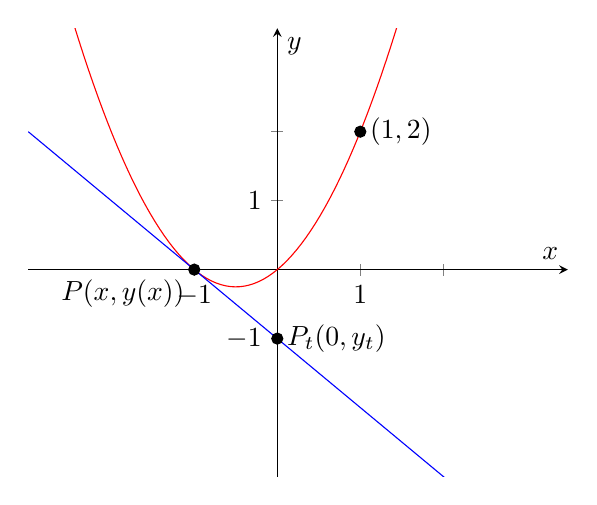
\begin{tikzpicture}
            \begin{axis}[
                axis lines = center,
                xlabel = \(x\),
                ylabel = \(y\),
                xmin = -3, xmax = 3.5,
                ymin = -3, ymax = 3.5,
                xtick = {-1, 1, 2},
                ytick = {-1, 1, 2},
                xticklabels = {\(-1\), \(1\)},
                yticklabels = {\(-1\), \(1\)},
            ]
            \addplot[domain=-2.5:2, samples=80, color=red]{x^2+x};

            % Marcamos el punto P(x, y(x))
            \addplot[mark=*] coordinates {(-1,0)} node[below left] {\(P(x, y(x))\)};

            % Marcamos la recta tangente
            \addplot[domain=-3:3, samples=2, color=blue]{-x-1};
            % Marcamos el punto de corte de la recta tangente con el eje de ordenadas
            \addplot[mark=*] coordinates {(0,-1)} node[right] {\(P_t(0, y_t)\)};

            % Marcamos el (1,2)
            \addplot[mark=*] coordinates {(1,2)} node[right] {\((1,2)\)};
            \end{axis}
        \end{tikzpicture}
        \caption{Representación gráfica del enunciado del Ejercicio~\ref{ej:2.2.10}.}
        \label{fig:ej:2.2.10}
    \end{figure}

    La distancia de un punto $P(x, y(x))$ al origen es $d(P, O)=\sqrt{x^2+y(x)^2}$, y la segunda coordenada del punto de corte de la recta tangente y el eje de ordenadas es $y_t$. Calculemos $y_t$ usando la definición de pendiente:
    \begin{align*}
        y'(x) &= \dfrac{y(x)-y_t}{x-0} \Longrightarrow y_t = -y'(x)x+y(x)
    \end{align*}
    Notemos además que, en el caso de $x=0$, se tiene que $y_t = y(x)$, por lo que se sigue teniendo. Como la condición impuesta por el enunciado es que $d(P, O)=y_t$, tenemos que:
    \begin{align*}
        \sqrt{x^2+y(x)^2} &= -y'(x)x+y(x) \qquad \text{con dominio }\bb{R}^3
    \end{align*}

    Expresando en forma normal, tenemos que:
    \begin{align*}
        y'=-\dfrac{\sqrt{x^2+y^2}-y}{x}
        =-\sqrt{1+\left(\dfrac{y}{x}\right)^2}+\dfrac{y}{x} \qquad \text{con dominio }\bb{R}^+\times \bb{R}
    \end{align*}
    Notemos que, al pasar a forma normal, hemos tenido que reducir el dominio. Optamos por los valores de $x$ positivos puesto que $(1,2)$ es un punto de la curva.\\

    Pasamos entonces a resolver la ecuación diferencial dada. Para ello, como se trata de una ecuación homogénea, aplicamos el cambio de variable:
    \Func{\varphi=(\varphi_1,\varphi_2)}{\bb{R}^+\times \bb{R}}{D_1}{(x,y)}{(x,z)=\left(x, \dfrac{y}{x}\right)}

    Veamos cuál es el codominio de $\varphi$:
    \begin{equation*}
        D_1=\varphi(D) = \left\{(x,z)\in \bb{R}^2 \mid (x, zx)\in D\right\} = \left\{(x,z)\in \bb{R}^2 \mid x>0 \right\}
        = \bb{R}^+\times \bb{R}
    \end{equation*}

    Tenemos que su inversa, por poder despejar de forma única cada componente, es:
    \Func{\varphi^{-1}}{D_1}{\bb{R}^+\times \bb{R}}{(x,z)}{(x,y)=(x, xz)}

    En primer lugar, tenemos que $\varphi,\varphi^{-1}$ son biyectivas, y al ser ambas componentes de clase $1$ (la segunda es producto o cociente de funciones de clase $1$), tenemos que $\varphi$ es un difeomorfismo. Además, es admisible por no variar la primera variable.

    Aplicando el cambio de variable a la ecuación dada, obtenemos:
    \begin{align*}
        \dfrac{dz}{dx} & = -\dfrac{y}{x^2} + \dfrac{y'}{x}
        = -\dfrac{z}{x} + \dfrac{-\sqrt{1+\left(\dfrac{y}{x}\right)^2}+\dfrac{y}{x}}{x} = \dfrac{-\sqrt{1+z^2}}{x} \qquad \text{con dominio }\bb{R}^+\times \bb{R}
    \end{align*}

    Esta ecuación es de variables separadas, y la función dependiente de $z$ no tiene soluciones constantes, luego aplicamos directamente el método:
    \begin{align*}
        \dfrac{dz}{\sqrt{1+z^2}} &= -\dfrac{dx}{x} \Longrightarrow \int \dfrac{dz}{\sqrt{1+z^2}} = -\int \dfrac{dx}{x} \Longrightarrow \operatorname{arcsenh}(z) = -\ln(x) + C \Longrightarrow\\&\Longrightarrow z = \senh(-\ln(x) + C) \qquad x\in \bb{R}^+
    \end{align*}

    Deshaciendo el cambio de variable, obtenemos la solución uniparamétrica de la ecuación dada:
    \begin{equation*}
        y(x) = x\senh(-\ln(x) + C) \qquad x\in \bb{R}^+
    \end{equation*}

    Usando la condición inicial $y(1)=2$, obtenemos:
    \begin{align*}
        y(1) &= \senh(-\ln(1) + C) = 2 \Longrightarrow \senh(C) = 2 \Longrightarrow \dfrac{e^C-e^{-C}}{2} = 2 \Longrightarrow e^C-e^{-C} = 4 \Longrightarrow\\&\Longrightarrow e^{2C}-1 = 4e^C \Longrightarrow (e^C)^2-4e^C-1 = 0 \Longrightarrow e^C = \dfrac{4+ \sqrt{16+4}}{2} = 2+ \sqrt{5} \Longrightarrow\\&\Longrightarrow C = \ln(2+ \sqrt{5})
    \end{align*}

    Por tanto, la solución de la ecuación dada que verifica $y(1)=2$ es:
    \begin{equation*}
        y(x) = x\senh(-\ln(x) + \ln(2+ \sqrt{5})) = x\senh\left(\ln\left(\dfrac{2+ \sqrt{5}}{x}\right)\right) \qquad x\in \bb{R}^+
    \end{equation*}
\end{ejercicio}

\begin{ejercicio}
    Identifique la clase de ecuaciones invariantes por el grupo de transformaciones $s = \lambda t$, $y = \lambda^2 x$, con $\lambda\in \bb{R}^+$.\\

    Consideramos un conjunto $D\subset \bb{R}^2$ abierto y conexo, una función continua $f:D\to \bb{R}$ y una ecuación diferencial de la forma:
    \begin{equation*}
        x' = f(t, x)
    \end{equation*}

    Consideramos ahora el cambio de variable dado por:
    \Func{\varphi_\lm=(\varphi_1,\varphi_2)}{D}{D}{(t,x)}{(s,y)=(\lambda t, \lambda^2 x)}

    Veamos qué condiciones hemos de imponer sobre el dominio $D$ para que sea este invariante por $\varphi$:
    \begin{equation*}
        D=\varphi(D) = \left\{(s,y)\in \bb{R}^2 \mid \left(\dfrac{s}{\lambda}, \dfrac{y}{\lambda^2}\right)\in D\right\} = \left\{(s,y)\in \bb{R}^2 \mid \left(\dfrac{s}{\lambda}, \dfrac{y}{\lambda^2}\right)\in D\right\}
    \end{equation*}
    % // TODO: Imponer condiciones sobre D

    Tenemos que su inversa, por poder despejar de forma única cada componente, es:
    \Func{\varphi_\lm^{-1}}{D}{D}{(s,y)}{(t,x)=(\nicefrac{s}{\lambda}, \nicefrac{y}{\lambda^2})}

    En primer lugar, tenemos que $\varphi_\lm,\varphi_\lm^{-1}$ son biyectivas, y al ser ambas componentes de clase $1$ por ser polinómicas, tenemos que $\varphi_\lm$ es un difeomorfismo. Además, es admisible ya que:
    \begin{equation*}
        \dfrac{\partial \varphi_1}{\partial t} + \dfrac{\partial \varphi_1}{\partial x}x' = \lambda + 0\cdot f(t,x) = \lambda\neq 0
    \end{equation*}

    Aplicando el cambio de variable a la ecuación dada, obtenemos:
    \begin{align*}
        \dfrac{dy}{ds} &= \dfrac{dy}{dt}\cdot \dfrac{dt}{ds} = \dfrac{dy}{dt}\cdot \dfrac{1}{\lambda} = \lm^2x'\cdot \dfrac{1}{\lambda} = \lm f(t,x) = \lm f\left(\dfrac{s}{\lm}, \dfrac{y}{\lm^2}\right) = \wh{f}(s,y)
    \end{align*}

    Por tanto, para que la ecuación sea invariante por el grupo de transformaciones dado, hemos de tener que:
    \begin{equation*}
        f(s,y) = \wh{f}(s,y) = \lm f\left(\dfrac{s}{\lm}, \dfrac{y}{\lm^2}\right) \qquad \forall(s,y)\in D,~\forall \lm\in \bb{R}^+
    \end{equation*}
    % // TODO: Imponer condiciones sobre f
\end{ejercicio}

\begin{ejercicio}
    Resuelva los problemas 42 y 45 (pag. 79) del libro de Nagle-Saff-Sneider.

    \begin{enumerate}
        \item \textbf{Problema 42:} Utilize la sustitución $y=ux^2$ para resolver la ecuación:
        \begin{equation*}
            \dfrac{dy}{dx} = \dfrac{2y}{x} + \cos\left(\dfrac{y}{x^2}\right)
        \end{equation*}

        % // TODO: Cont Arturo
        
        \item \textbf{Problema 45: [Ecuaciones Acopladas]} Al analizar ecuaciones acopladas de la forma
        \begin{align*}
            \dfrac{dy}{dt} &= ax+by,\\
            \dfrac{dx}{dt} &= \alpha x+\beta y,
        \end{align*} 
        donde $a,b,\alpha,\beta$ son constantes, quisiéreamos determinar la relación entre $x$ e $y$ en vez de las soluciones individuales $x(t)$, $y(t)$. Para hacer esto, divida la primera ecuación entre la segunda para obtener:
        \begin{equation*}
            \dfrac{dy}{dx} = \dfrac{ax+by}{\alpha x+\beta y}
        \end{equation*}
        Esta nueva ecuación es homogénea, de modo que podemos resolverla mediante la sustitución $u=\nicefrac{y}{x}$. Nos referimos a sus soluciones como \emph{curvas integrales}. Determine las curvas integrales del sistema:
        \begin{align*}
            \dfrac{dy}{dt} &= -4x-y,\\
            \dfrac{dx}{dt} &= 2x-y.
        \end{align*}

        % // TODO: Cont Arturo
    \end{enumerate}
\end{ejercicio}